% 压缩浮动体之间的间距
\setlength{\floatsep}{4pt plus 2pt minus 2pt}
\setlength{\textfloatsep}{6pt plus 2pt minus 2pt}
\setlength{\intextsep}{4pt plus 2pt minus 2pt}
\setlength{\abovecaptionskip}{3pt}
\setlength{\belowcaptionskip}{2pt}

\section{实验结果}

首先介绍我们的实验设置，对于SVM的训练方案，手势前后补充样本数量为100；对于基于CNN和频谱RGB图像的方案，采用MobileNet v2（在ImageNet 1K上预训练）进行全量微调，优化器使用Adam优化器；对于LSTM方法，采用input size=6, hidden\_size=60，同样采用Adam优化器，具体参数配置如下。

\begin{table}[h!]
    \centering
    \caption{\ptheadingfont{SVM训练配置}}
    \label{tab:svm_config}
    {\zihao{5}\setlength{\baselineskip}{1\baselineskip}%
    \begin{tabularx}{\linewidth}{|>{\centering\arraybackslash}p{3cm}|>{\centering\arraybackslash}p{2cm}|>{\centering\arraybackslash}X|>{\centering\arraybackslash}p{2cm}|}
        \hline
        \textbf{输入特征} & \textbf{填充Padding} & \textbf{分类器} & \textbf{Epoch} \\
        \hline
        41维（3$\times$13+2） & 100 & SVC(kernel=``rbf'', C=5)\newline + OneVsRestClassifier & 无epoch \\
        \hline
    \end{tabularx}}
\end{table}

\begin{table}[h!]
    \centering
    \caption{\ptheadingfont{CNN训练配置}}
    \label{tab:cnn_config}
    {\zihao{5}\setlength{\baselineskip}{1\baselineskip}\setlength{\tabcolsep}{3pt}%
    \begin{tabularx}{\linewidth}{|>{\centering\arraybackslash}p{1.5cm}|>{\centering\arraybackslash}p{2.8cm}|>{\centering\arraybackslash}p{2.0cm}|>{\centering\arraybackslash}p{1.0cm}|>{\centering\arraybackslash}X|>{\centering\arraybackslash}p{2.0cm}|>{\centering\arraybackslash}p{0.9cm}|}
        \hline
        \textbf{输入维度} & \textbf{骨干网络} & \textbf{批次大小} & \textbf{优化器} & \textbf{优化器参数} & \textbf{学习率调度} & \textbf{Epoch} \\
        \hline
        $224\times224$ & MobileNetV2\newline (ImageNet~1K) & Train:8~/\newline Val:16 & Adam & LR=3e-4,\newline WD=1e-4 & step=10,\newline gamma=0.5 & 30 \\
        \hline
    \end{tabularx}}
\end{table}

\begin{table}[h!]
    \centering
    \caption{\ptheadingfont{LSTM训练配置}}
    \label{tab:lstm_config}
    {\zihao{5}\setlength{\baselineskip}{1\baselineskip}\setlength{\tabcolsep}{3pt}%
    \begin{tabularx}{\linewidth}{|>{\centering\arraybackslash}p{1.5cm}|>{\centering\arraybackslash}p{3.0cm}|>{\centering\arraybackslash}p{1.4cm}|>{\centering\arraybackslash}p{1.0cm}|>{\centering\arraybackslash}X|>{\centering\arraybackslash}p{2.0cm}|>{\centering\arraybackslash}p{0.9cm}|}
        \hline
        \textbf{隐藏维度} & \textbf{网络结构} & \textbf{批次大小} & \textbf{优化器} & \textbf{优化器参数} & \textbf{损失函数} & \textbf{Epoch} \\
        \hline
        60 & LSTM(6,60)$\to$\newline Linear(60,\newline num\_classes) & 10 & Adam & LR=3e-3,\newline WD=2e-3 & CrossEntropy\newline Loss & 30 \\
        \hline
    \end{tabularx}}
\end{table}

我们的测试结果如下所示，其中，SVM方法平均训练时间0.011s，CNN方法平均训练时间172.1s，LSTM平均训练时间为79.1s。

\begin{table}[h!]
    \centering
    \caption{\ptheadingfont{SVM vs. CNN vs. RNN/LSTM}}
    \label{tab:results}
    {\zihao{5}\setlength{\baselineskip}{1\baselineskip}\setlength{\tabcolsep}{3pt}%
    \begin{tabularx}{\linewidth}{|>{\centering\arraybackslash}p{0.8cm}|*{4}{>{\centering\arraybackslash}X}|*{4}{>{\centering\arraybackslash}X}|*{4}{>{\centering\arraybackslash}X}|}
        \hline
        & \multicolumn{4}{c|}{\textbf{SVM}} & \multicolumn{4}{c|}{\textbf{CNN}} & \multicolumn{4}{c|}{\textbf{LSTM}} \\
        \hline
        \textbf{Fold} & Acc & Prec & Rec & F1 & Acc & Prec & Rec & F1 & Acc & Prec & Rec & F1 \\
        \hline
        1 & 91.2 & 89.5 & 87.2 & 88.1 & 99.1 & 98.8 & 99.3 & 99.0 & 63.2 & 58.1 & 50.0 & 52.0 \\
        2 & 92.9 & 91.5 & 90.2 & 90.5 & 98.2 & 97.4 & 99.3 & 98.3 & 61.1 & 65.0 & 48.6 & 49.9 \\
        3 & 86.7 & 87.6 & 84.8 & 85.6 & 97.3 & 98.0 & 96.9 & 97.4 & 60.2 & 57.7 & 48.9 & 49.4 \\
        4 & 90.3 & 88.9 & 87.1 & 87.8 & 99.1 & 98.7 & 98.6 & 98.6 & 64.8 & 63.2 & 50.9 & 50.8 \\
        5 & 89.4 & 90.3 & 86.1 & 87.5 & 98.2 & 99.3 & 97.4 & 98.2 & 63.7 & 67.6 & 52.4 & 54.9 \\
        \hline
        \textbf{Avg.} & \textbf{90.1} & \textbf{89.6} & \textbf{87.1} & \textbf{87.9} & \textbf{98.4} & \textbf{98.5} & \textbf{98.3} & \textbf{98.3} & \textbf{62.5} & \textbf{62.3} & \textbf{50.2} & \textbf{51.4} \\
        \hline
    \end{tabularx}}
\end{table}

其中对于LSTM这种方法呈现的意外低准确率作出以下分析：1.数据量太小，而LSTM参数量较大，可能导致过拟合；2.时序长度不稳定，当前的样本中的手势信号为了确保鲁棒性，在样本前段的静止时间并非固定，而LSTM高度依赖固定的时序模板，进行时间归一化后可能已经破坏时序依赖，这也证明了LSTM方法在手势识别任务中并没有达到理想效果。相比LSTM对长时间依赖关系的建模，频谱图中的局部纹理与边缘结构更适合由卷积核进行空间特征提取，因此CNN表现出显著优势。

对原始 I/Q 时域信号进行 STFT 频域变换得到频谱图后，不同类别的频谱图呈现出肉眼可见的差异，同类别的频谱图则具有相似的时频结构，这为基于 CNN 的二维图像分类提供了可解释性依据。如图~\ref{fig:umap_clustering}和图~\ref{fig:spectrogram_grid}所示：

\begin{figure}[htbp]
    \centering
    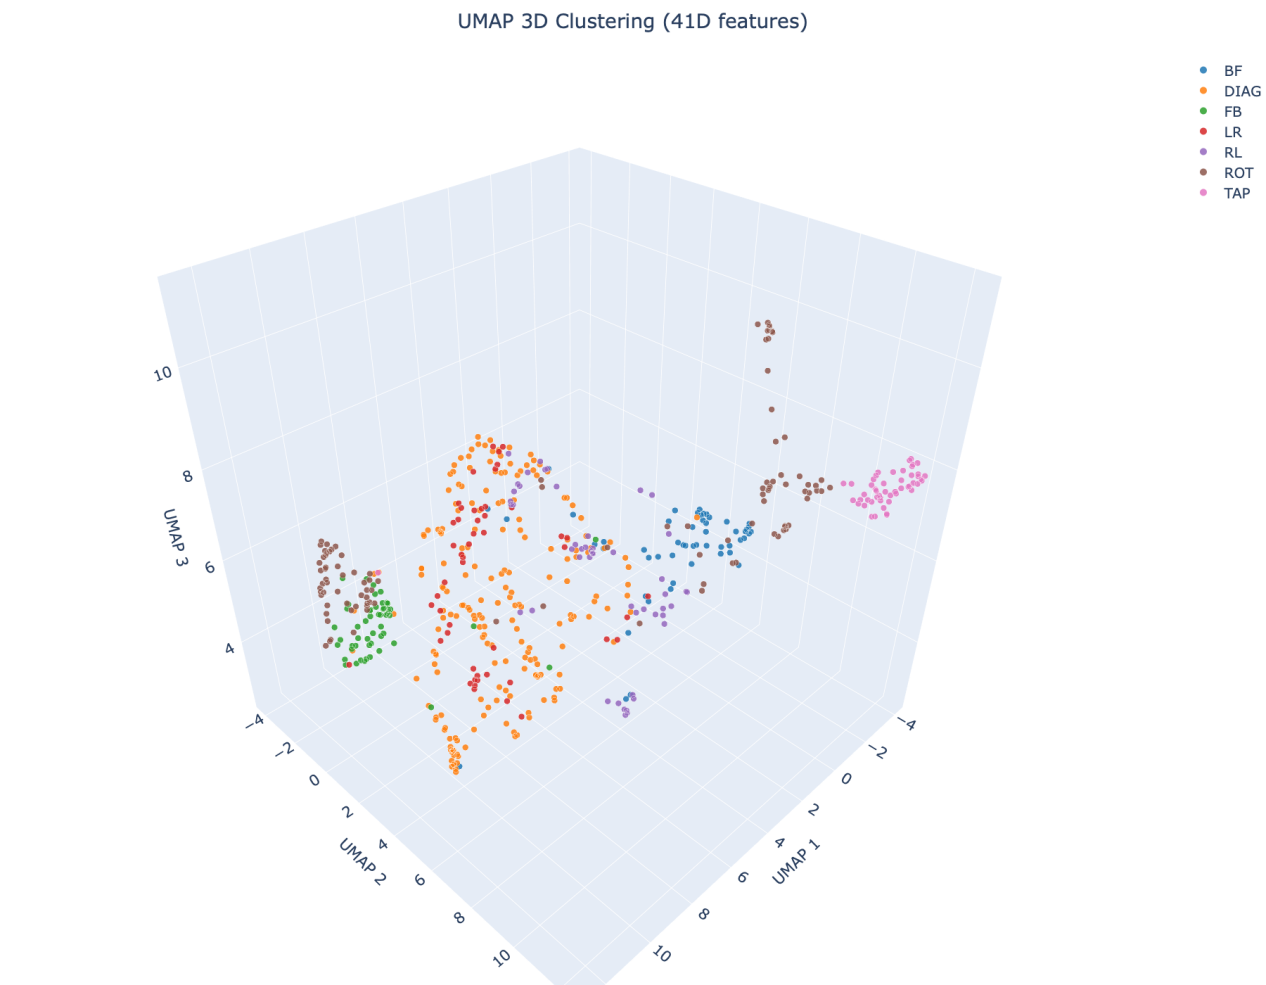
\includegraphics[width=0.85\textwidth]{doc_thesis/figs/04/umap_clustering.png}
    \caption{\ptheadingfont{SVM确定性信号聚类图}}
    \label{fig:umap_clustering}
\end{figure}

\begin{figure}[htbp]
    \centering
    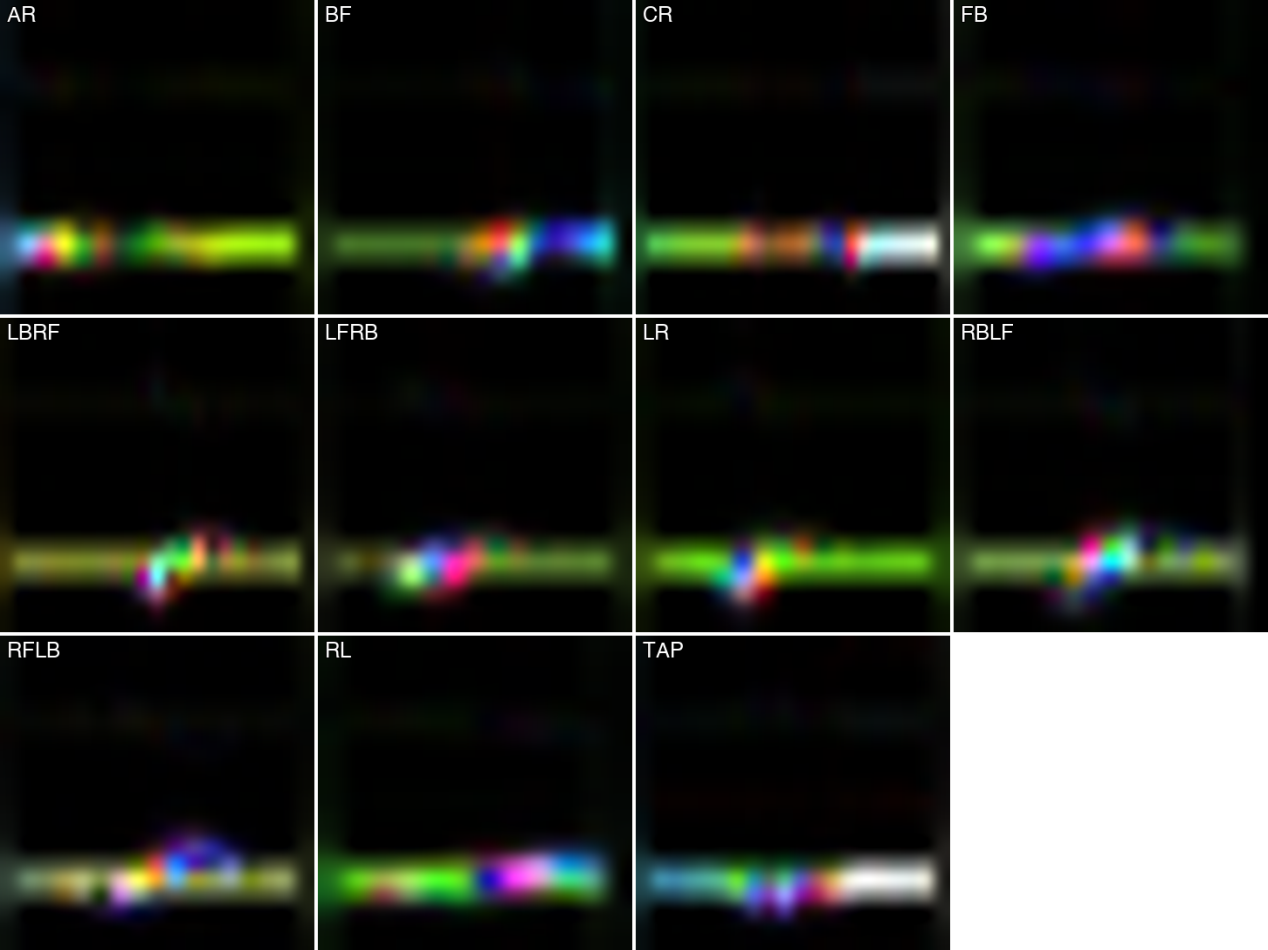
\includegraphics[width=0.85\textwidth]{doc_thesis/figs/04/spectrogram_grid.png}
    \caption{\ptheadingfont{手势信号混色频谱图}}
    \label{fig:spectrogram_grid}
\end{figure}

我们发现，对于非平动（比如转动），SVM系统的鲁棒性非常弱，尤其体现在确定性信号上，这与我们之前的理论分析相符合，也就是物理波长限制了对于微手势的识别，散射特性对角度极其敏感，相位特征稳定性下降。

\begin{figure}[htbp]
    \centering
    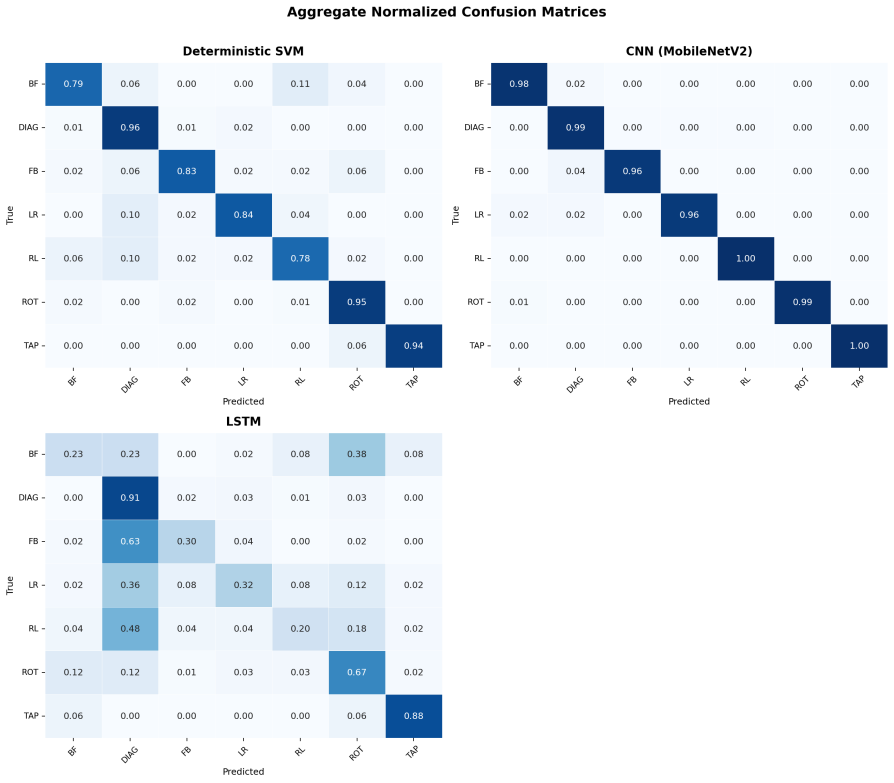
\includegraphics[width=0.7\textwidth]{doc_thesis/figs/04/confusion_matrices.png}
    \caption{\ptheadingfont{三种方法混淆矩阵对比图}}
    \label{fig:confusion_matrices}
\end{figure}

CNN 的混淆矩阵呈对角占优，大多数类别的识别准确率超过96\%，其中 R 类与 TAP 类达到100\%，说明微多普勒频谱图的局部纹理与时频结构能够被卷积核有效提取。LSTM 出现较多非对角元素，说明时序特征在当前数据规模和表示下未被充分学习。SVM 未采用深度特征学习，平均识别准确率仍达到90\%以上，说明基于确定性多普勒相位构建的低维特征向量具有较强的类别可分性。

SVM 的主要混淆集中于运动方向相近的类别之间：L 与 R 的频谱在频移方向上具有近似镜像关系，B 与 F 在时间反演后频谱结构相似，是两类主要的混淆来源。

不同手势在雷达视角下会产生不同的径向速度变化过程，因此其对应的微多普勒谱图在频率扩展范围、能量聚集区域以及时间演化轨迹上呈现出具有物理意义的差异。这说明频谱图不仅是神经网络输入，更反映了手部运动学与电磁散射之间的映射关系。

同时对比已有的研究成果，Cai et al.\cite{Cai_2019} 曾提出，在使用57–64GHz、2Tx4Rx FMCW 雷达，提取 range、speed、azimuth 三类轨迹，并合成为 128×128×3 的 RSA 输入送入 CNN的情况下，在 ResNet-20 模型中达到了最高的98.7 \% 的准确；相比于我们的TDM-SIMO方案效能相近，但是Cai 选用的数据集是 50 名受试者、4 类手势、3652 条有效记录，并通过随机裁剪增强到 40 万+训练样本，成本更高，系统更加复杂，当前模式提出的方案更具低成本可实施性。

相比于 Latern\cite{Latern}采用 24GHz FMCW雷达 将连续雷达回波转换为谱图序列，并通过 3D-CNN、LSTM 和 CTC 的组合实现未分割连续手势流识别。其核心优势在于 CTC 能够在不预先标注手势起止点的情况下对手势核心阶段进行对齐和分类，因此在连续手势识别任务中达到 96.25\% 的准确率。相比之下，本文主要面向低成本 5.8GHz 连续波 TDM-SIMO 雷达平台，系统无法直接获得 FMCW 雷达中的高分辨率距离维信息，因此更关注从多通道 I/Q、相位和功率峰值中提取低维确定性特征，并结合 SVM 实现轻量分类。本文 CNN 方法在较小数据规模下达到 98.4\%，说明即使缺少 FMCW 距离维信息，微多普勒频谱图仍具有较强判别能力；而 SVM 方法达到 90.1\%，训练时间仅 0.011s，体现出端侧部署优势。虽然在连续手势识别场景下并没有足够的实验证明，但是足以证明当前方法在单手势识别中的效果。

综合来看，确定性信号+SVM准确率90.1\%，训练时间仅0.011s，模型体积小，可在CPU上运行；CNN准确率最高（98.4\%），但训练耗时172.1s，内存占用约1GB；LSTM各项指标均最低，主要原因是小样本场景（每类50--60样本）下过拟合，以及时序归一化破坏了时序依赖结构。

\section{研究展望}

基于本研究的实验结果与局限性分析，后续研究方向聚焦在以下几个方面：

\begin{enumerate}[itemsep=0pt, parsep=0pt, topsep=0pt, partopsep=0pt]
    \item 当前确定性信号方法对旋转类手势（AR/CR）识别效果有限，原因是旋转运动产生的相位曲线非单调，不具备确定性极值时序特征。可探索将幅度包络的时频特征与相位确定性特征进行融合，构建更完备的手势表征，以扩展对非平动手势的识别能力。
    \item 将米氏散射模型的几何约束（如相位演化凸性、极值点拓扑关系）作为正则项引入轻量神经网络，在保持物理可解释性的同时提升对复杂手势的泛化能力，使物理先验与数据驱动方法形成互补。
    \item 当前数据集规模较小（每类约50--60样本），限制了CNN和LSTM的跨用户泛化能力。可针对新用户或新手势的快速适配需求，探索小样本学习方案，降低采集成本。
    \item 5.8\,GHz波长（约5.2\,cm）与手掌尺寸相当，处于米氏散射敏感区，散射特性对照射角度变化较为敏感。引入更高频段（如24\,GHz）可缩短波长、降低散射对角度的敏感性，有望改善对细粒度手势的识别效果；亦可探索双频联合感知以兼顾穿透性与分辨率。
    \item 雷达信号本身不直接采集图像，对用户隐私较为友好，但高精度回波仍可能反映用户行为规律。后续可研究在特征提取阶段引入隐私保护机制，进一步明确系统在隐私敏感场景下的适用边界。
\end{enumerate}

\section{结论}

毕业设计以三通道TDM-SIMO连续波多普勒雷达为硬件平台，围绕非接触式手势识别的理论建模、系统实现与算法设计三方面展开研究，完成了预期目标中的各项核心任务。

首先从米氏散射理论出发，分析了手掌在近场条件下的动态反射散射特性，推导了手掌运动与各通道接收信号之间的确定性相位关系。基于反正弦解调算法提取的多普勒累积相位及其功率峰值时刻具有明确的物理含义，实验结果表明确定性信号方法在11类手势上的平均分类准确率达到90.1\%。

随后搭建硬件链路实现了稳定的高速采样，算法端构建了三种互补的识别方案：确定性信号特征+SVM训练时间仅0.011s，推理延迟约0.33ms；CNN迁移学习方案达到了98.4\%的最高准确率，推理延迟约6ms；两者均满足实时交互要求。系统完成了对平动（前后、左右、点击）、对角线冗余及旋转共11类手势的分类评估。

针对连续交互场景中缺乏严格静止段的问题，通过连续信号流自动回溯静止区间恢复直流基线，并以功率峰值时间替代相位最小值特征，将确定性信号方法在该场景下的准确率从约15\%提升至90.1\%。

综上，本研究从物理建模到系统实现再到算法优化，完成了5.8\,GHz TDM-SIMO多普勒雷达手势识别系统的设计与验证，三种分类方案在准确率、训练效率和资源消耗上各有侧重，可根据实际部署场景灵活选用。
